% Introduction

\section{Scope of this study}

Not much is known about knowledge sharing mechanisms in open innovation. This study examines tacit knowledge sharing behaviour in three open innovation projects. Particular attention is given to tacit knowledge. 


 because tacit knowledge  because it is considered vital for innovation. The study considers knowledge sharing behaviour in terms of power-relations and personal motivation. 



Particular attention is given to relative differences in absorptive capacity between open innovation partners 

Firms are finding it harder to compete in the knowledge-based economy. They can no longer rely solely on their internal knowledge-base to remain competitive. Not surprisingly, a growing number of firms are embracing open innovation as a competitive strategy. Not only does this allow them to access external knowledge resources, it also enables them to profit from internally developed knowledge by making it available to other firms \citep{laursen2006open,chesbrough2013managing,stanko2017under}. Despite mounting evidence on the potential benefits of open innovation, little is known about knowledge sharing practices in open innovation \citep{lakemond2016match}. This study attempts to fill this gap by examining the individual, organisational, and managerial antecedents of knowledge sharing in three open innovation projects. Particular attention is given to tacit knowledge sharing, a vital ingredient for successful innovation \citep{leonard1998role,koskinen2002role,cavusgil2003tacit,seidler2008use,leonard2014knowledge}.

\section{Background}

\subsection{Defining innovation}

Innovation may be defined as \enquote{the development and implementation of new ideas by people who, over time, engage in relationships with others within an institutional and environmental context} \citep[][pg.]{van1986central}. Insofar an idea is perceived as new to the people involved, it is an innovation even though it may appear to others as nothing more than an imitation of something that exists elsewhere \citep{van1986central}. Innovation is essentially about the renewal of the business in order to remain competitive and enhance its ability to create value \citep{schumpeter1950capitalism}. Failure to innovate places a firm's ability to survive and prosper at risk \citep{bessant2005managing}.

\subsection{Trend towards open innovation}

The ever-increasing technical complexity of products, processes, and services demands levels of knowledge beyond what most firms possess or can develop in a market-relevant time-frame. Many firms are turning to open innovation as a competitive strategy \citep{enkel2009open,bessant2013innovation}. Open innovation depends on a wide network of inter-organisational relationships to access new external knowledge and exploit novel ideas \citep{chiaroni2010unravelling}. While tapping into external knowledge resources is not a new idea \citep{mowery2009plus,trott2009open}, open innovation is not just about accessing external knowledge. Rather, it should be seen as a manifestation of the relational view of competitive advantage \citep{dyer1998relational}. The relational view is an extension of the resource-based view of the firm, which argues a firm's competitive advantage stems from the application of tangible and intangible resources available to it \citep{wernerfelt1984resource,peteraf1993cornerstones}. Sustained competitive advantage can be achieved if these resources are valuable, rare, inimitable, and non-substitutable \citep{barney1991firm}. The knowledge-based view treats knowledge as the most strategically important resource of a firm and emphasizes the importance of having effective processes for transferring knowledge across organisational boundaries \citep{kogut1992knowledge,drucker1994post,grant1996toward}. Understanding how these processes deliver competitive advantage requires a relational view that focuses on the social structures, routines, and processes for knowledge exchange \citep{dyer1998relational}. The relational view argues firms can generate relational rents jointly with alliance partners \citep{dyer1998relational,lavie2006competitive}. This is exactly what open innovation is all about. \medskip

Open innovation is formally defined as a distributed innovation process based on carefully managed knowledge flows across firm boundaries using mechanisms as per the firm's business model\footnote{The term \enquote{business model} is defined as \enquote{the chosen system of inputs, business activities, outputs and outcomes that aims to create value over the short, medium, and long term} \citep{gould2013business}}. The business model helps a firm determine which inflows of knowledge can fuel innovation, and which knowledge should be released to other organisations \citep{chesbrough2017future}. Put differently, the business model explains how relational rents can be generated through knowledge sharing. \medskip

Key benefits of open innovation include early access to new technology, sharing of risk, reduced costs of development, better customer acceptance of products or services, and enhanced ability to continuously innovate \citep{ye2013exploring}. Because distributed innovation processes are hard to observe and imitate, open innovation is a useful strategy for sustaining competitive advantage \citep{barney1991firm,lichtenthaler2011open}. \medskip

Open innovation also facilitates more radical innovation \footnote{Innovations can be classified as either incremental or radical \citep{henderson1990architectural}. Incremental innovation is a series of small improvements or upgrades made to a firm's existing products, services, processes, or methods. Radical innovation supplants these with something entirely new, potentially disrupting an existing market or economic activity of other firms operating in that market \citep{leifer2001implementing,mcdermott2002managing}. Each type of innovation requires different resources and core competencies to have any effect \citep{lam2000tacit,darroch2002examining}. Incremental innovations do not require a significant departure from current business practices and are likely to enhance existing internal competencies by providing the opportunity for those within the organisation to build on existing know-how. Radical innovations, on the other hand, are likely to be competence-destroying, often making existing skills and knowledge redundant \citep{tushman1986technological}. This has implications for knowledge management in terms of finding the balance between seeking out new and unfamiliar knowledge, and building on an existing knowledge base \citep{march1991exploration}.} \citep{inauen2012fostering,engen2014radical}.\medskip

%  The business model explains how the firm uses its dynamic capabilities to capture value from its strategic collaborations \citep{chesbrough2002role,teece2010business,ziegler2013creating,durst2013success}. 

% Relational rents are extracted from relation-specific assets, knowledge-sharing routines, complementary resources, and effective governance mechanisms \citep{lavie2006competitive}.

% Firms in open innovation systems need dynamic capabilities to internalise and externalise knowledge to gain competitive advantage \citep{ziegler2013creating}. 

\subsection{Open innovation processes}

Open innovation can be described in terms of inbound, outbound and coupled innovation processes \citep{chesbrough2006beyond,enkel2009open,gassmann2010future}. Figure \ref{fig:oi_process} illustrates how these processes may work in practice. \enquote{Inbound open innovation} enriches a firm’s knowledge base through integrating suppliers, customers and other external actors \citep{xu2013inbound} while \enquote{outbound open innovation} refers to the commercial exploitation of knowledge that has been developed in-house \citep{de2016knowledge}. \enquote{Coupled open innovation} focuses on strategic alliances that encompass both inbound and outbound innovation processes \citep{spithoven2013open}. \medskip

\begin{figure}
	\centering
	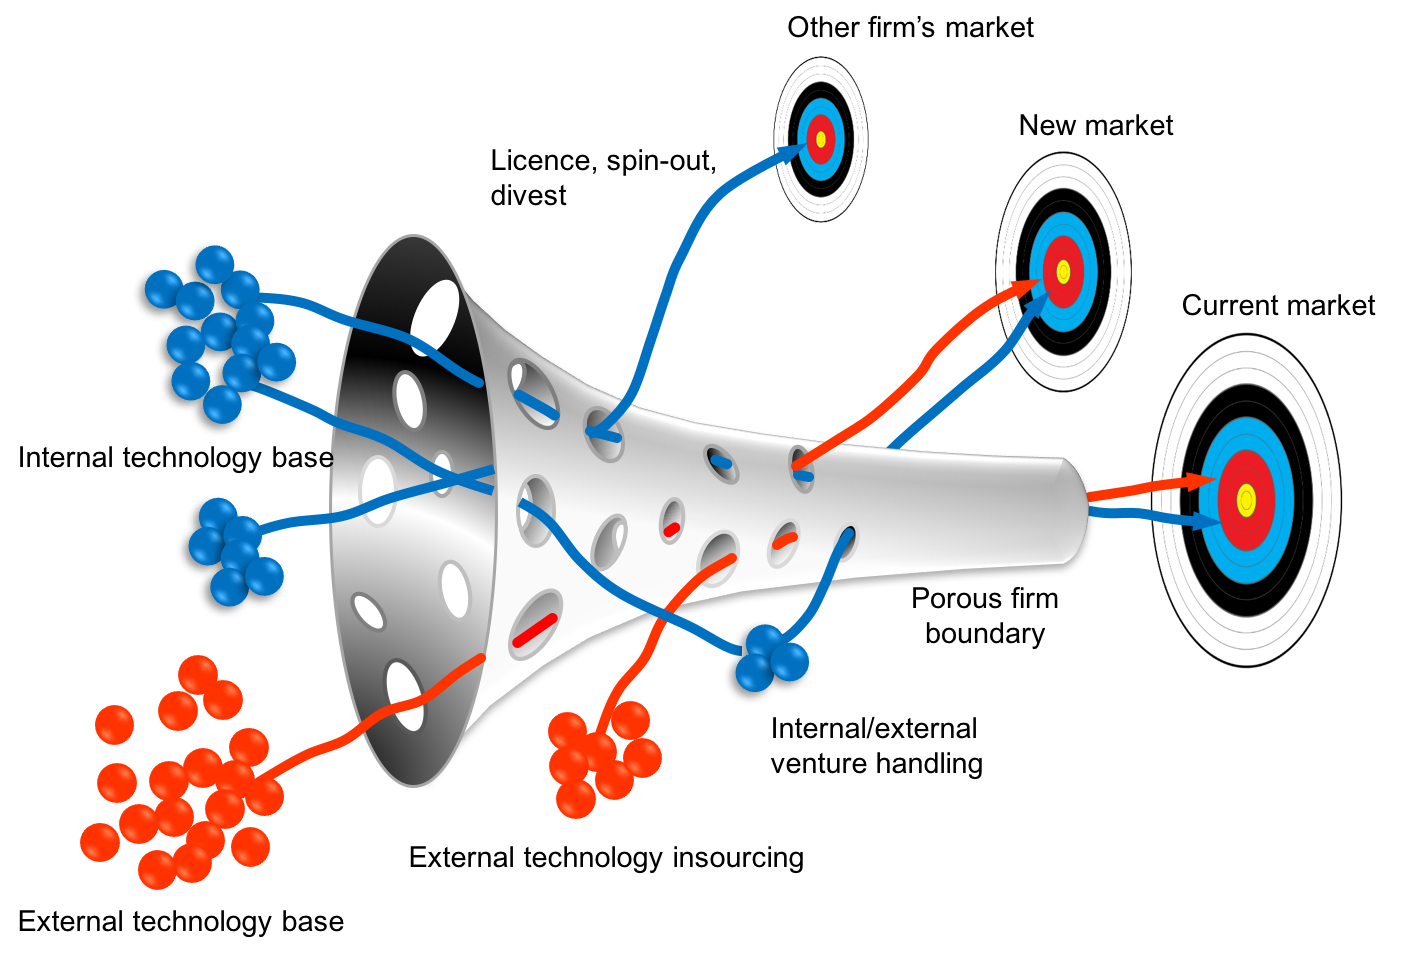
\includegraphics[width=0.9\linewidth]{Images/oi_process}
	\caption{Open innovation processes \citep{chesbrough2004open}. Image courtesy of SlideModel.}.
	\label{fig:oi_process}
\end{figure}

\subsection{Challenges of open innovation}

For all its benefits, open innovation still presents firms with numerous management challenges \citep{hossain2013open,vanhaverbeke2014surfing}. These include transforming the firm's business model to support open innovation, changing internal approaches to research and development, building a more open culture, identifying suitable organisations to partner with, and protecting intellectual property, to name but a few \citep{dahlander2010open,sieg2010managerial,lichtenthaler2011your,durst2013success,roper2013externalities,aloini2016structured}. Managing knowledge flows in open innovation is particularly challenging because the locus of innovation resides not within a firm, but in a network of social relations that span organisational boundaries \citep{powell1996interorganizational,elmquist2009exploring}. Factors that influence the communication of knowledge across organisational boundaries include 

\subsubsection{Relative differences in absorptive capacity}

Absorptive capacity is defined as the \enquote{ability of a firm to recognise the value of new, external information, assimilate it, and apply it to commercial ends} \citep{cohen1990absorptive}. Firms need absorptive capacity to properly engage in open innovation \citep{vanhaverbeke2007connecting}. Relative differences in absorptive capacity can impede the flow of knowledge across firm boundaries, create power imbalances, undermine alliance performance, and result in less favourable open innovation outcomes \citep{szulanski1996exploring,lane1998relative,nooteboom2000learning,vanhaverbeke2007connecting,easterby2008absorptive,phelps2012knowledge}. Reducing the cognitive distance between partner organisations is a key challenge in open innovation \citep{nooteboom2000learning,vanhaverbeke2007connecting}. \medskip

\subsubsection{Communicating tacit knowledge}

Much of the knowledge possessed by individuals and groups is tacit, held either in people's minds or in the form of unwritten rules or practices that guide the collective action of groups \citep{mowery1996strategic,leonard1998role,burt2007secondhand,goksel2016can,lichtenthaler2016absorptive}. \medskip

Explicit and tacit knowledge should not be treated as a dichotomy, but rather as a spectrum with the two knowledge types at each extreme \citep{polanyi1966tacit,inkpen1998knowledge,cavusgil2003tacit}. At one end of the spectrum, knowledge is almost completely tacit, embodied in the minds and experience of people. At the other end of the spectrum, knowledge is almost completely explicit, existing in codified or structured form and accessible to other people \citep{leonard1998role}. Some describe the knowledge resource available to a firm as an iceberg. Explicit knowledge is the visible tip of the iceberg where the knowledge resource is easy to recognise and access. Hidden beneath the surface is the vast bulk of the iceberg, symbolising tacit knowledge derived from a lifetime of experience, practice, perception and learning \citep{haldin2000difficulties,mcadam2007exploring,rebernik2007fostering}. Because it is largely invisible, tacit knowledge is a tremendous source of competitive advantage \citep{nelson1982evolutionary,barney1991firm,grant1996toward,smith2001role,chilton2007dimensions,lu2015job}.\medskip

Tacit knowledge is considered critical for innovation as it guides the thought processes that produce novel ideas \citep{leonard1998role,amar2008descriptive}. The most common application of tacit knowledge is problem-solving. For instance, people with expertise from experience not only are able to recognise the situation in which they find themselves in, but also know which actions might be appropriate for dealing with it \citep{simon1971human,leonard1998role}. Tacit knowledge can also be used to reformulate problems by viewing these differently in intuitive ways. Intuition can also help predict or anticipate outcomes \citep{leonard1998role}. Managing the flow of tacit knowledge across organisational boundaries is confounded by the fact that tacit knowledge sharing cannot be mandated but happens through volition or free will \citep{polanyi1966tacit}. 

Unless acted upon, tacit and explicit knowledge is simply a latent resource. Knowledge becomes valuable when enacted in practice, symbolising the very act of knowing \citep{cook1999bridging,duguid2005art,marabelli2014knowing,freeman2015knowledge}. The management challenge is to orchestrate social interactions to facilitate tacit knowledge exchange and allow knowledge to be enacted in practice \citep{haldin2000difficulties,lankilaa2005knowledge}.

The processes described by \citet{nonaka1995knowledge} and \citet{crossan1999organizational} highlight the importance of social mechanisms for transferring individual learning to the organisational level. People in tight-knit groups are more likely to work with tacit knowledge in the form of unwritten yet mutually understood language and routines used to coordinate actions. However, tacit knowledge held within such groups is prone to being discounted or misunderstood by others \citep{burt2007secondhand}. This emphasises the need for people in boundary spanning roles to aid the transfer of diverse and often complex knowledge between groups \citep{tushman1981boundary,allen1984managing,szulanski2003sticky,seidler2008use,meyer2010rise,chesbrough2012open}.

\subsubsection{Brokering productive relationships}

Boundary spanners play a key role in open innovation as they facilitate the translation, integration and combination of unfamiliar and distant knowledge \citep{tushman1981boundary,allen1984managing,,meyer2010rise,chesbrough2012open}. They also broker new relations between otherwise disconnected actors in different organisational networks \citep{granovetter1973strength,burt2004structural,burt2007secondhand}. Efforts to create or widen existing inter-organisational networks may be frustrated by people reluctant to form new ties, facilitate third-party ties, or otherwise change their existing networks \citep{davis2010agency}. Not-invented-here and not-shared-here (also referred to as not-sold-here) syndromes can also stymie knowledge exchange \citep{lichtenthaler2006attitudes,lichtenthaler2011your,de2014neither,podmetina2015skills,chesbrough2017future}. Not-invented-here syndrome refers to resistance within a firm against externally developed knowledge \citep{katz1982investigating,hussinger2011search,antons2015opening}. Not-shared-here syndrome is a negative attitude towards external exploitation of internally developed knowledge assets \citep{chesbrough2003open,lichtenthaler2006attitudes,de2014neither}. Formation of productive relationships that allow knowledge to be combined in unique and valuable ways is contingent on overcoming resistance to...

 reluctance to form such resistance to allow the emergence of productive relationships that allows knowledge to be combined in unique and valuable ways \citep{uzzi1997social,nahapiet1998social,obstfeld2005social,lane2006reification,davis2010agency,meyer2010rise}.\medskip


\section{Research opportunity}

% measuring ACAP hard. Recent reserach points to practice-based approach. However these are time-consuming, laborious. SNA useful


Innovation is a socially intensive process that involves creative individuals who share knowledge and co-create ideas within a group \citep{leonard1998role}. How well this process works depends on the absorptive or learning capacity of individuals, groups, and firms \citep{cohen1989innovation}. Even though tacit knowledge is considered vitally important for innovation \citep{leonard1998role,cavusgil2003tacit,rebernik2007fostering,seidler2008use}, it has received scant attention in the open innovation literature.

Absorptive capacity is a complex multidimensional and somewhat abstract construct that is difficult to quantify or assess in practice. Little is known about the social practices that build absorptive capacity and how these are affected by tacit knowledge \citep{tortoriello2015social,lichtenthaler2016absorptive}. Recent studies have indicated that a practice-based approach is appropriate for identifying the routines and practices that build absorptive capacity \citep{duchek2013capturing,omidvar2013revisiting,marabelli2014knowing}. A practice-based approach usually involves embedding somebody within a firm to perform an ethnographic study \citep{duchek2013capturing}, which is intrusive, time-consuming, prone to observer bias, and hard to generalise \citep{goodson2011overview}. An alternative approach to assess how absorptive capacity emerges in practice is through applying mixed methods social network analysis. Mixed method social network analysis presents an opportunity to assess absorptive capacity across multiple levels of the boundary-crossing organisation, offering rich insights into the social complexity of absorptive capacity. \medskip 




\section{



There is a limit to what social-network analysis can tell us about social practices. New knowledge tends to be generated within a particular context, such as a product of observation or rich interactions that help individuals think about problems and solutions in a new context \citep{nonaka1994dynamic,wenger2000communities,cross2015investing}. Social network analysis needs to be complemented by a qualitative study to capture the context in which knowledge sharing and idea generation occurs. \medskip

Mixed method social network analysis presents an opportunity to assess how knowledge is enacted in practice and what this means in terms of building absorptive capacity and deleivering successful open innovation outcomes. \medskip 

\section{Study objectives}

This study employs mixed methods social network analysis to assess absorptive capacity processes within three open-innovation collaborations. Attention is focussed on psychological and social factors that govern knowledge-sharing behaviour and how these might influence tacit-knowledge exchange. \medskip

The overarching research question in this study is \enquote{how do psychological and social factors shape the development of absorptive capacity in open innovation?}. This question is answered by addressing three sub-questions:\medskip

\begin{enumerate}
	\item To what extent does autonomous motivation predict knowledge sharing behaviour? How is this affected by the level of tacit knowledge being exchanged?
	\item How do patterns of brokerage differ according to the level of tacit knowledge being shared? What does this reveal about the nature of the collaboration, and what does this tell us about power-relations?
	\item To what extent does the level of tacit knowledge exchange predict the emergence of novel ideas, and what does this reveal about the complexity of the innovation challenge? 
\end{enumerate}

The mixed methods social network analysis uses statistical modelling to assess how individual attributes, such as level of personal motivation, educational background, and work experience, influence the emergence of knowledge-sharing connections. The modelling also exposes patterns of social interaction operating across multiple levels \citep{monge2003theories,lusher2012exponential}. The modelling is complemented by semi-structured interviews that capture the industrial, organisational, and cultural contexts governing the emergence of collaborative social structures.\medskip 

\section{Research contribution}

This study advances knowledge in two ways. Firstly, the study provides fresh insight into how tacit knowledge shapes absorptive capacity and contributes to the success of open innovation. Secondly, it tests the feasibility of using social-network analysis to assess how absorptive capacity emerges in practice. Such analysis offers some advantages over a practice-based approach based on ethnography in terms of objectivity, generalisability, and time. By highlighting key social mechanisms that build absorptive capacity in collaborative innovation, this study contributes to more effective and practical ways to create and capture value from inter-organisational relationships.\medskip

\section{Document structure}

This document is organised into ten chapters. Chapter Two explains how the concept of absorptive capacity has evolved into a dynamic capability encompassing cognitive and behavioural change. This suggests that any assessment of absorptive capacity needs to consider what factors contribute to cognitive and behavioural change. \medskip

Chapter Three explains what social networks are and introduces key psychological and social theories that can be used to assess knowledge sharing behaviour. The mixed method research methodology used in this study is presented in Chapter Four. This includes a detailed description of the multi-theoretical multilevel-analytical framework used to assess the dynamic nature of absorptive capacity. \medskip

Chapter Five highlights the distinguishing characteristics of the three open-innovation case studies. Results from the mixed method social network analysis are presented separately for each case in Chapters Six, Seven, and Eight. Comparisons between the three sets of results are discussed in Chapter Nine. \medskip 

Finally, Chapter Ten summarises the key findings of this study and reflects on some key lessons learned as this study unfolded. 